\documentclass{sig-alternate}
%\setcounter{tocdepth}{3}
\usepackage{hyperref}
\usepackage[stable]{footmisc}
\usepackage{epsfig}
\usepackage{textcomp}
\usepackage{times}
\usepackage{amssymb}
\setcounter{tocdepth}{3}
\usepackage{graphicx}
\usepackage{url}
\usepackage{listings}
\usepackage{comment}


\setlength{\columnsep}{6.2mm}
\newcommand{\ie}{i.e.} 
\newcommand{\eg}{e.g.} 
\newcommand{\et}{et al. }
\begin{document}

%\conferenceinfo{}{ Portugal}
%\CopyrightYear{2014} 
%\crdata{978-1-4503-2627-8/14/07\\
%http://dx.doi.org/10.1145/XXXX}  

\title{SMAS: A Smart Meter Data Analytics System}

\numberofauthors{3}
\author{
\alignauthor
Xiufeng Liu \\
\affaddr{University of Waterloo}\\
\email{xiufeng.liu@uwaterloo.ca}
\alignauthor 
Lukasz Golab \\
\affaddr{University of Waterloo}\\
\email{lgolab@uwaterloo.ca}
\alignauthor 
Ihab F. Ilyas \\
\affaddr{University of Waterloo}\\
\email{ilyas@uwaterloo.ca}
}
\maketitle
\begin{abstract}

\end{abstract}
Smart meter data analysis is the key for energy consumers and suppliers to manage energy. In this paper, we present a smart meter data analytics system, SMAS, that can assist both  demand-side and supply-side energy management. Energy consumers can view their own energy consumption at different granularity levels of time dimension, and use feedback to monitor their energy usages. Utilities in SMAS can tackle the energy management problems, including customer load analysis, segmentation, consumpation pattern discovery, and forecasting. In the demonstration, conference attendees can interact with SMAS as the role of energy consumer or provider, and see a variety of analyses on a real-world electricity dataset.

%\category{A.m}{General}{Miscellaneous}
%\category{H.2.m}{Database Management}{Miscellaneous}

%\keywords{Smart Meter data, Aanlysis, System}

\section{Introduction}
Smart meter is an advanced meter that measures the energy consumption of  consumers. Smart meters read the real-time energy usage at a regular interval (usually every 15 minutes or hourly), which  produces a large amount of fine-grained data. This provides utilities the opportunity to use the data to improve the way they run the grid, \ie, analyze meter data, and turn it into actionable insights. However, smart meters are  new, and until now, leveraging smart meter data has not been as common as the traditional  technologies in the market. For example, residential users are not able to view their recent energy usage, but have to wait till the billing date,  typically once per month. They also could not see the detailed energy consumption data via a web browser, but the aggregated usage in the monthly paper report. For energy providers such as utility companies, they have little knowledge in using smart meters analytics, and  using the analysis in infrastructure planning, network optimization, and designing effective demand-response programs.  These necessities studying smart meter data technologies, and creating the analytics platform. Currently, some smart meter data platforms are available, but most are offered by commercial companies, such as SAP \footnote{www.sap.com/pc/tech/in-memory-computing-hana/software/ smart-meter-analytics/index.html}, Oracle/Data Raker \footnote{www.oracle.com/us/products/applications/utilities/meterdata-analytics/index.html}, and the start-ups, such as Autogrid.com, C3Energy.com and OPower.com. It is not clear what algorithms were implemented and the technologies were used and how. Jarrah Nezhad \et implemented the open source SmartD \cite{jarrah}, which  is a smart meter data analytics dashboard with limited functionalities.


In this paper, we present a prototype system for smart meter data analysis, named {\em SMAS}, which is built incorporating our recent benchmarking results of smart meter data analytics \cite{benchmarking}. This system supports meter data analysis of both demand-side and supply-side, and aims to support real-time analysis using  data streams from smart meters.  For the demand-side analysis, SMAS supports  consumer to view their own consumption data at different granularity levels of time  dimension, compare their load profile with the peer users, and monitor their consumption by feedback service. For the supply-side analysis, SMAS supports discovering the consumption patterns of customers by using data mining techniques. Based on the found patterns, SMAS can segment customers with precision based on the patterns using clustering techniques. SMAS can predict energy consumption on different temporal aggregations.  In this prototype, we have so far concentrated on validating our methods in the residential sector of electricity, which in itself presents many challenges, but our techniques should work in commercial and industrial sectors, and also work for our planning water data analysis.
\begin{figure*}[htp]
\vspace{-5pt}
\begin{minipage}[b]{0.55\linewidth}
\centering
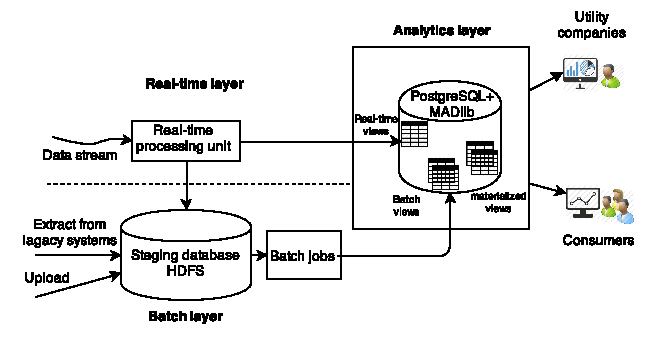
\epsfig{file=images/architecture, scale=0.8}
\vspace{-5pt}
\caption{System architecture}
\label{fig:architecture}
\end{minipage}
\hspace{5pt}
\begin{minipage}[b]{0.45\linewidth}
\centering
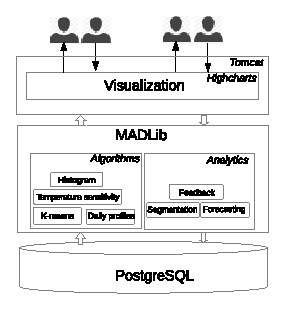
\epsfig{file=images/analyticslayer, scale=1.0}
\vspace{-10pt}
\caption{Analytics Layer}
\label{fig:analyticslayer}
\end{minipage}
\vspace{-25pt}
\end{figure*}

\section{System Overview}
This system is under development. We envision our system in production will support the analytics of both real-time and static data. We thus propose the system architecture shown in Figure~\ref{fig:architecture}.   This architecture is able to handle both real-time data streams from smart meters and the data from legacy systems, \eg, the systems of storing the traditional scalar meter data or from the upload. The architecture consists of three layers: {\em batch layer,  real-time layer} and {\em analytics layer}.  The batch layer is responsible for generating the views from the large data sets in the batch-layer database, and writes the output to the analytics layer database. The batch job runs repeatedly, and the batch views in the analytics layer are outdated when new batch views have been generated, \ie, the old batch views will be overridden. In the meantime of two sequential batch view updates, a parallel real-time layer constantly processing the most recent data, and updates the real-time views in analytics layer. Therefore, users can query the most recent data as well as the stale data by merging the batch views and the real-time views. The real-time layer also writes the data into the batch-layer database, in which the data will be included with the other existing data and processed by the next batch job. We envision that data streaming systems, such as S4, Spark or Storm, will be used in our real-time layer, and Hive (with the underlying Haddop distributed file system and MapReduce) will be used as the batch-layer database, and runs the batch jobs.  The analytics layer consists of a high performance database, analytics libraries, web application and report engine which are together to serve users' queries. So far we have implemented the analytics layer, which uses the open source relational DBMS, PostgreSQL, as the analytics-layer database,  MADLib \cite{madlib} as the in-database analytics library, Highcharts (www.highcharts.com) as the visualization engine, and Tomcat as the web application server (see Figure~\ref{fig:analyticslayer}). The implemented analytics modules include load analysis, pattern discovery, segmentation, forecasting and feedback services. The future extensions  may include using the PostgreSQL-XL cluster (www.postgres-xl.org) for  big data workload,  applying columnar store to PostgreSQL (citusdata.github.io/cstore\_fdw), and the support for R, and Matlab. 




\section{Analytics Algorithms}
{\bf Histogram.} It is important for utilities to know the consumption variability of consumers in order to provision the peak demand and to provide incentives to flatten the peak; For consumers, it is also important to learn their own consumption distribution so as to adjust their living habits to reduce the demand of high energy consumption. The simplest way to understand the consumption of variability  is to use the histogram to compute the distribution of consumption for each consumer. The chart at top right in Figure~\ref{fig:patterndiscovery} shows an example of hourly consumption distribution (Y-axis) over various ranges within a period of time (X-axis). 

{\bf 3-Line Algorithm.} Electricity consumption is often sensitive to the change of outdoor temperatures, \eg, the consumption rises with the decreasing of temperature in cold weather (due to heating) and the increasing of temperature in warm weather (due to cooling).  In SMAS, we use 3-line algorithm \cite{birt} to study the effect of the outdoor temperatures to the electricity consumption of a consumer. In the scatter plot of the points between the consumptions and  outdoor temperatures, the algorithm uses three piecewise regression lines to fit the points  (see Figure~\ref{fig:threelmodel}, the algorithm connects the three lines by adjusting the lines slightly). The upper three regression lines are computed for the points in the 90th percentile for each temperature value, while the lower three lines are computed for the points in the 10th percentile  for each temperature value. 3-line algorithm  profiles the load into the following four constituents for customer feedback  (also shown in  Figure~\ref{fig:threelmodel}): 1) heating and cooling gradient, which correspond to the slopes of the left and right 90th percentile lines. A high heating and cooling gradient value might be caused by using inefficient heating and  cooling systems (or using cooling systems at a low temperature setpoint); 2) base load, which is the height at the lowest point of the 10th percentile lines. It is the consumption of the appliance that are always on regardless of outdoor temperatures, such as refrigerators; 3) activity load, which is the height between the lowest point on the 90th percentile lines and base load. It is the consumption due to household activities, such as using  washing machines, dishwashers, ovens, lights, TV, etc. 
\begin{figure}[htp]
%\vspace{-5pt}
\centering

\includegraphics[width=0.35\textwidth]{images/threelmodel}
\vspace{-8pt}
\caption{3-line regression model}
\label{fig:threelmodel}
\vspace{-10pt}
\end{figure}

{\bf PARX Algorithm.} It is interesting for utilities to learn  daily consumption trend in order to provision daily energy supply. We use the PARX algorithm (periodic auto-regression with eXogenous variables) \cite{omid} to extract the daily consumption trend regardless of the outdoor temperature. 
 The idea behind this algorithm is shown in Figure~\ref{fig:dailyprofile}. At the left, we show a fragment of the hourly consumption time series for some consumer over a period of several days. We are only given the total hourly consumption, but the goal of the algorithm is to determine, for each hour, how much load is temperature-independent and how much additional load is due to temperature (i.e., heating or cooling). Once this is determined, the algorithm computes the average temperature-independent consumption at each hour of the day, illustrated at the right of Figure~\ref{fig:dailyprofile}.
\begin{figure}[htp]
\vspace{-10pt}
\centering
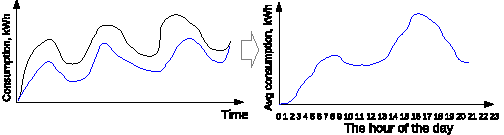
\includegraphics[width=0.5\textwidth]{images/dailyprofile}
\vspace{-20pt}
\caption{3-line regression model}
\label{fig:dailyprofile}
\vspace{-10pt}
\end{figure}

For each consumer and the hour of a day at $t$, \ie, $t=0...23$, the algorithm takes the consumptions at $t$ of the previous $p$ days, and the corresponding outdoor temperatures (the exogenous variable) as the input, then uses auto-regression model to compute the coefficients. Finally, the algorithm computes the activity load by removing the load caused by temperatures from the total load  using the computed coefficients.

\begin{comment}
Another load disaggregation metric used in SMAS is the daily average load profile regardless of the outdoor temperature. This is to study the daily consumption trend of a household. We compute the average load profile at 0--23 o'clock (or called {\em season}) over a period of several days. The model of time-series periodic auto-regression with eXogenous variables (PARX) \cite{omid} is used in the computation. The model has considered the recent history values of an order $p$ (\ie, the most recent $p$ data points at time $t$), and the exogenous variables such as weather temperature and the characteristics of a property. PARX is defined as: 
\begin{equation}
Y_t = \Sigma_{i=1}^p \phi_{i}Y_{t-i}  + \Sigma_{j=1}^n \psi_{j}X_t^j + C_s +  \epsilon_{t},   t \in s
\end{equation}
where $Y_t$ is the time-series value at the time $t$; $\phi_{i}$ is the auto-regression parameter up to the order $p$; $X^j$ and $\psi_j$ are the exogenous variable and the corresponding coefficient, respectively; $C_s$ is a seasonally varying intercept term, and $s$ is the season index;  $\epsilon_{t}$ is a standard white noise at the time $t$ with zero mean and variance $\sigma$. The parameters of the model are estimated using Ordinary Least Squares (OSL). Then, the new time series of removing  the value owned by exogenous variables are computed by $Y_t^* = Y_t - \Sigma_{j=1}^n \phi_{j}X_t^j$. In the end, we compute the hourly averages corresponding to $Y_t^*$s for the weekdays and weekends/holidays, respectively. The bottom chart of Figure~\ref{fig:loadprofiling} has shown the result of the average daily profile of weekdays (black line) and weekends/holidays (blue line) of a household.
\end{comment}

{\bf Clustering Algorithm.} Consumers with similar consumption patterns can be identified by using  clustering algorithms. We use by far the most popular clustering algorithm, K-means, which typically uses Euclidean distance between elements in the cluster, \ie, $d(X, Y)= \sqrt{\sum_{i=1}^{n}(x_i-y_i)^2}$, where $X=(x_1, x_2, ..., x_n)$ and $Y=(y_1, y_2, ..., y_n)$.



\section{The Application}
SMAS offers  different views with a different functionality for the use of consumers and utilities.

\subsection{Consumer Views}
{\bf My Consumption.}
In the view of my  consumption (see Figure~\ref{fig:loadanalysistimeseries}, consumers can explore their own consumption data at different granularities at time dimension, \ie, hourly, daily, weekly or monthly. At the finest granular level, the system displays the raw time-series data of the hourly resolution. While, at higher granular levels, the system returns the summarized  data, \eg, The blue area plot in Figure~\ref{fig:loadanalysistimeseries} shows the aggregated daily usage of a consumer. 

{\bf Feedback Service.}
Feedback service allows energy consumers to set the rules of receiving alert messages. For example, users can set the feedback service based on the results of comparing their own consumption with the average of peer users. Once it is set, the system will automatically send messages with a pre-set  interval. Due to the privacy reason, one can only compare with the average of many  consumers, \eg, the consumers of living in the same street, same area, or selected from Google Map.  For example, Figure~\ref{fig:loadanalysistimeseries} shows the comparison of a consumer's daily load (the blue area plot) against the average of living in the same street (the yellow area plot). By comparing against  the peers, one can find the root cause to improve  energy efficiency. For example, if the consumption is higher than expected relative to its peers, (s)he may discover that this is due to air conditioners not being set to a higher temperature during nights or using  inefficient air conditioners. 


\subsection{Utilities Views}
{\bf Consumption Analysis.}  Utilities can view the consumption at different granularities with respect to the dimensions of time and geographic location, and view the aggregated consumption with respect to the functions, {\em sum, average, min} or {\em max}.  Utilities can also compare the consumption of any two individuals or feed areas. The user interface is similar to Figure~\ref{fig:loadanalysistimeseries}, but allows users to choose the aggregation functions and geographic locations.  

{\bf Consumption Pattern Discovery.}
Smart meter time-series data reflects the load influenced by various factors, such as consumer indoor activity, outdoor weather temperature, and the appliances used. Consumption pattern discovery can help utilities to better understand the consumption practices of customers so that they can provide customers appropriate recommendations for energy saving. In pattern discovery, SMAS can display  not only the raw time-series data (see Figure~\ref{fig:loadanalysistimeseries}), but also the load shapes disaggregated by the 3-line and PARX algorithms (see  Figure~\ref{fig:patterndiscovery}). From the chart at the top left in Figure~\ref{fig:patterndiscovery}, utilities are able to learn the base load, activity load, heating gradient and cooling gradient of a customer. The bottom chart displays the daily average load profile of a customer regardless of the outdoor temperatures in weekday (blue line) and weekend/holiday (black line), respectively. Utilities can learn the hourly consumption distribution of a customer from the chart at the top right in Figure~\ref{fig:patterndiscovery}.


{\bf Segmentation.}
For utilities, one of the most important tasks is to segment  customers according to their  energy consumption and load profiles. Customer segmentation can be used to carry out  more precise marketing communication with the customers, \eg, to promote the most appropriate energy-savings programs to a targeted segment. In SMAS, utilities can cluster customers based on extracted consumption features, including base load, activity load, heating and cooling gradients; and the daily load profile of customers; and the shapes of average load over a day, a week or a month. The segmentation is proceeded by using K-means clustering algorithm. To segment customers who have similar load shapes, \eg, over a period of time, we first normalize the load at each of the time series by dividing the total load of that period, then segment them by running the clustering algorithm. Figure~\ref{fig:segmentation} shows an example of customer segmentation, which classifies customers into three segments according to their base load using Euclidean distance. The top chart displays the centroids of the clusters, each of which indicates the distribution of the count of consumers over the ranges of base load. The bottom chart shows the Map locations of customers of each cluster, indicated by a different color. By clicking the legend on the top chart, users can toggle the visibility of a cluster shown on both charts.

{\bf Forecasting.}
The energy industry is reliant on balancing energy supply and demand, and thus requires to predict customer energy consumption. For instance, by predicting the periods of peak demand, utilities can avoid distribution failure by upgrading the infrastructure for more capacity, use dynamic pricing to incentivize customers to lower energy usage during peak times, and provide customers the recommendation of shifting from the peaks.  SMAS supports doing the following forecasts: individual household forecasting, feed area, and the overall forecasting at the time granularity of daily, weekly, and monthly. SMAS has integrated the forecast algorithms, including PARX, ARIMA, and exponential smoothing HoltWinters (the screenshot is not shown due to space reason). 



\section{Demonstration}
We will demonstrate the functionalities of SMAS through the hands-on interaction with conference attendees. Our goals are two\-fold: 1) demonstrate  our system in surfacing charts of smart meter data analysis; 2) share energy management knowledge from the perspectives of energy suppliers and consumers. We will use the real-world dataset, the electricity consumption data of 27,300 households
% in Southwestern Ontario, Canada between 2011 and 2012 at an hourly time resolution 
(roughly 10GB). We will demonstrate our system to the attendees using the following two scenarios.

{\bf Scenario 1 (Energy Consumer).} An attendee is provided a consumer account, and logs in. In my consumption view, she browses her electricity usage at the granularity of hourly, daily, weekly or monthly, and views the statistics data about how many hours/days at various ranges of usage in the past. She might be interested in comparing her own consumption with her neighborhood. She, then, chooses to compare  any other consumers on Google Map (or the neighborhoods living in the same street, region, or all areas), and compares her daily/weekly/monthly consumption with the average. She can set to receive the usage feedback when she is in over consumption. She, then, goes to the feedback tab to set the rules, \eg, set for receiving message when her consumption is 30\% higher than the average of the neighbors of the same street.

{\bf Scenario 2 (Energy Provider).}
An attendee is provided a utilities account, and logs in. In the consumption analysis tab, she views the consumption of an individual household/feed area/all by the time granularity of hourly/daily/weekly/monthly. In the pattern discovery tab, she dis-aggreg\-ates the load of a customer with regard to the base load, activity load, daily load profile with respect to weekdays and weekends/holidays. She segments the consumers in terms of the profiled load with K-means clustering algorithm, and view the difference of the results shown on the charts of centroids and Map when using different distance metrics.  In forecasting, she predicts the energy consumption at the level of individual household/feed area/all, and chooses different forecasting algorithms to see the difference of forecasting results. Finally, in the feedback service tab, she  sets the rules for the consumers who will receive the feedback messages according to the pattern of energy consumption, \eg, the customers whose the daily base load exceeds 10 kWh will receive alert messages.
 
\noindent {\bf Acknowledges.} The research is supported by IBM Canada Research and Development Centre and SOSCIP.org. 



\raggedright
\flushleft
\begin{thebibliography}{20}
{\small
\bibitem{omid}
O.~Ardakanian, N.~Koochakzadeh, R.~P.~Singh, L.~Golab, and S.Keshav. Computing Electricity Consumption Profiles from Household Smart Meter Data. In Proc. of EnDM, 2014.

\bibitem{birt}
B.~J.~Birt, G.~R.~Newsham,  I.~Beausoleil-Morrison, M.~M.~Armstrong,  N.~Saldanha, and I.~H.~Rowlands. Disaggregating Categories of Electrical Energy End-use from Whole-house Hourly Data. Energy and Buildings, 50, pp.~93--102, 2012.

\bibitem{madlib}
 J.~M.~Hellerstein, C.~R\'{e}, F.~Schoppmann, D.~Wang, E.~Fratkin, A.~Gorajek, and A.~Kumar. The MADlib Analytics Library: or MAD Skills, the SQL. PVLDB, 5(12):1700--1711, 2012.

\bibitem{jarrah}
A.~Jarrah Nezhad, T.~K.~Wijaya, M.~Vasirani, and K.~Aberer.  SmartD: Smart Meter Data Analytics Dashboard. In Proc. of e-Energy, 2014.

\bibitem{benchmarking}
X.~Liu, L.~Golab,  and I.~Ilyas. Benchmarking of Smart Meter Data Analytics. In Submission, 2014.

}

\end{thebibliography}

\appendix
\begin{figure*}[htp]
\centering
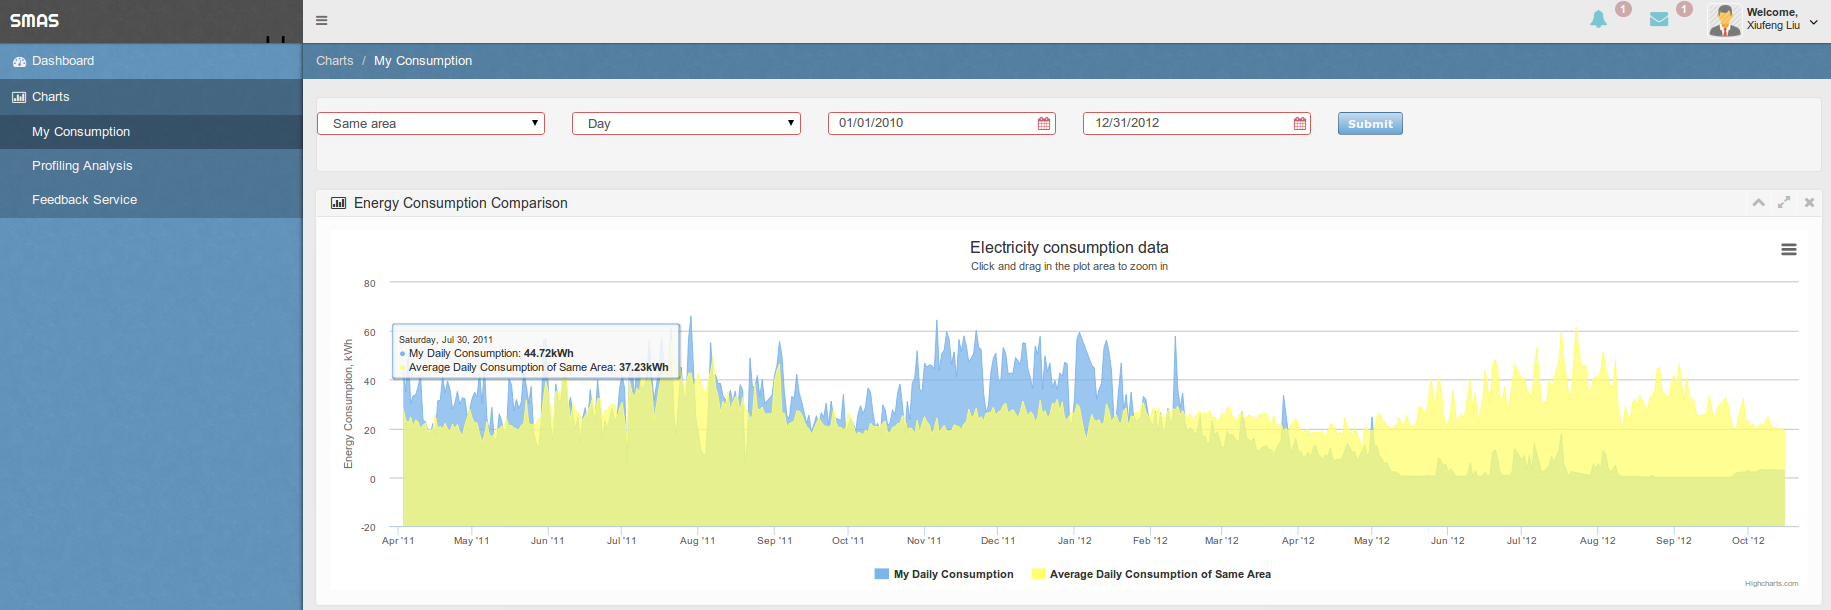
\includegraphics[width=0.82\textwidth]{images/loadanalysistimeseries}
\vspace{-15pt}
\caption{Consumption analysis}
\label{fig:loadanalysistimeseries}
\vspace{-5pt}
\end{figure*}
\begin{figure*}[htp]
\centering
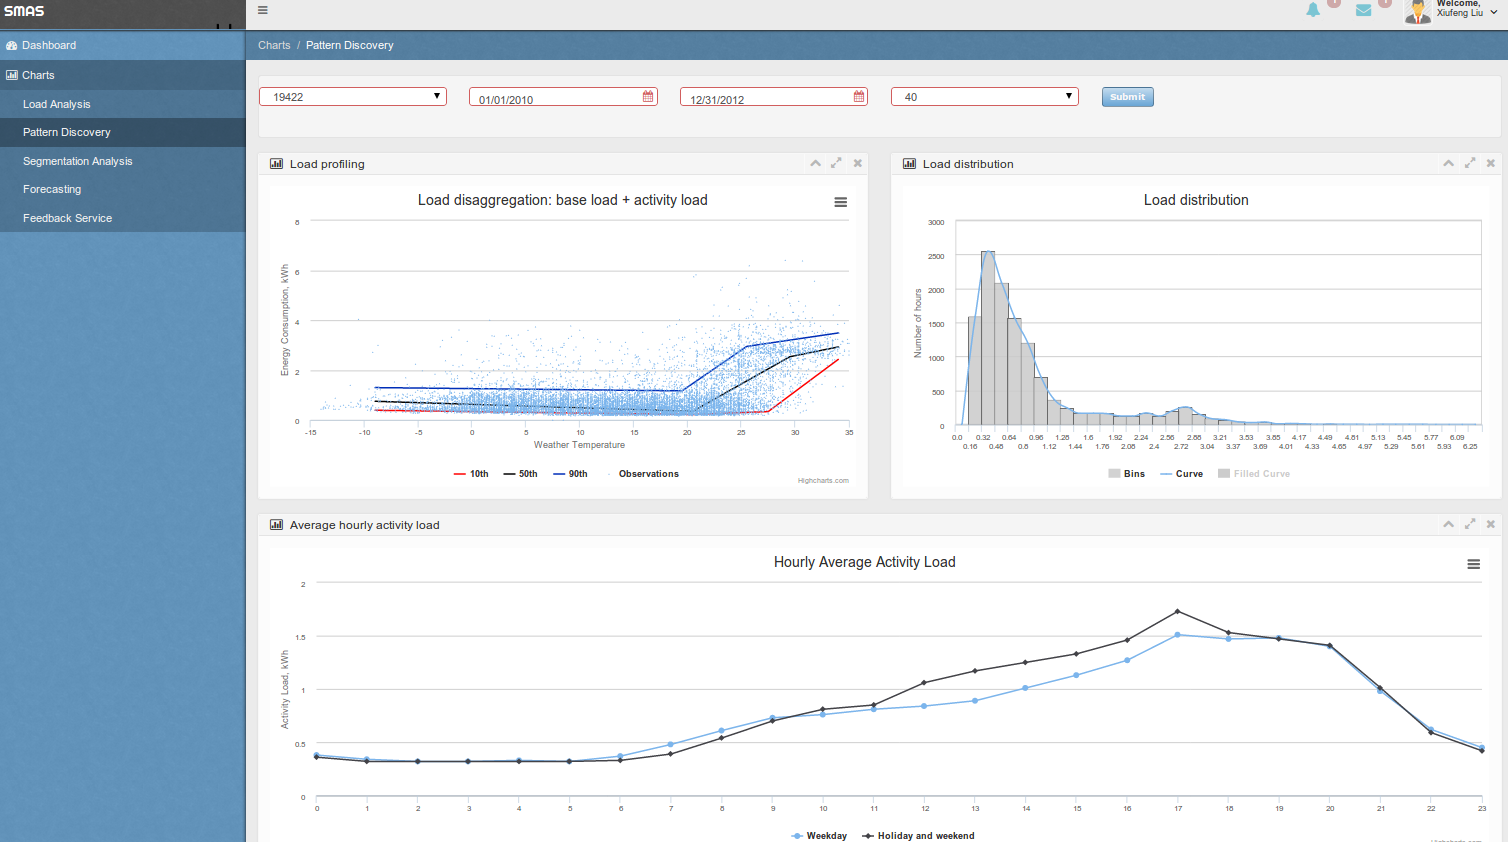
\includegraphics[width=0.82\textwidth]{images/patterndiscovery}
\vspace{-15pt}
\caption{Consumption pattern  discovery}
\label{fig:patterndiscovery}
\vspace{-5pt}
\end{figure*}
\begin{figure*}[htp]
\centering
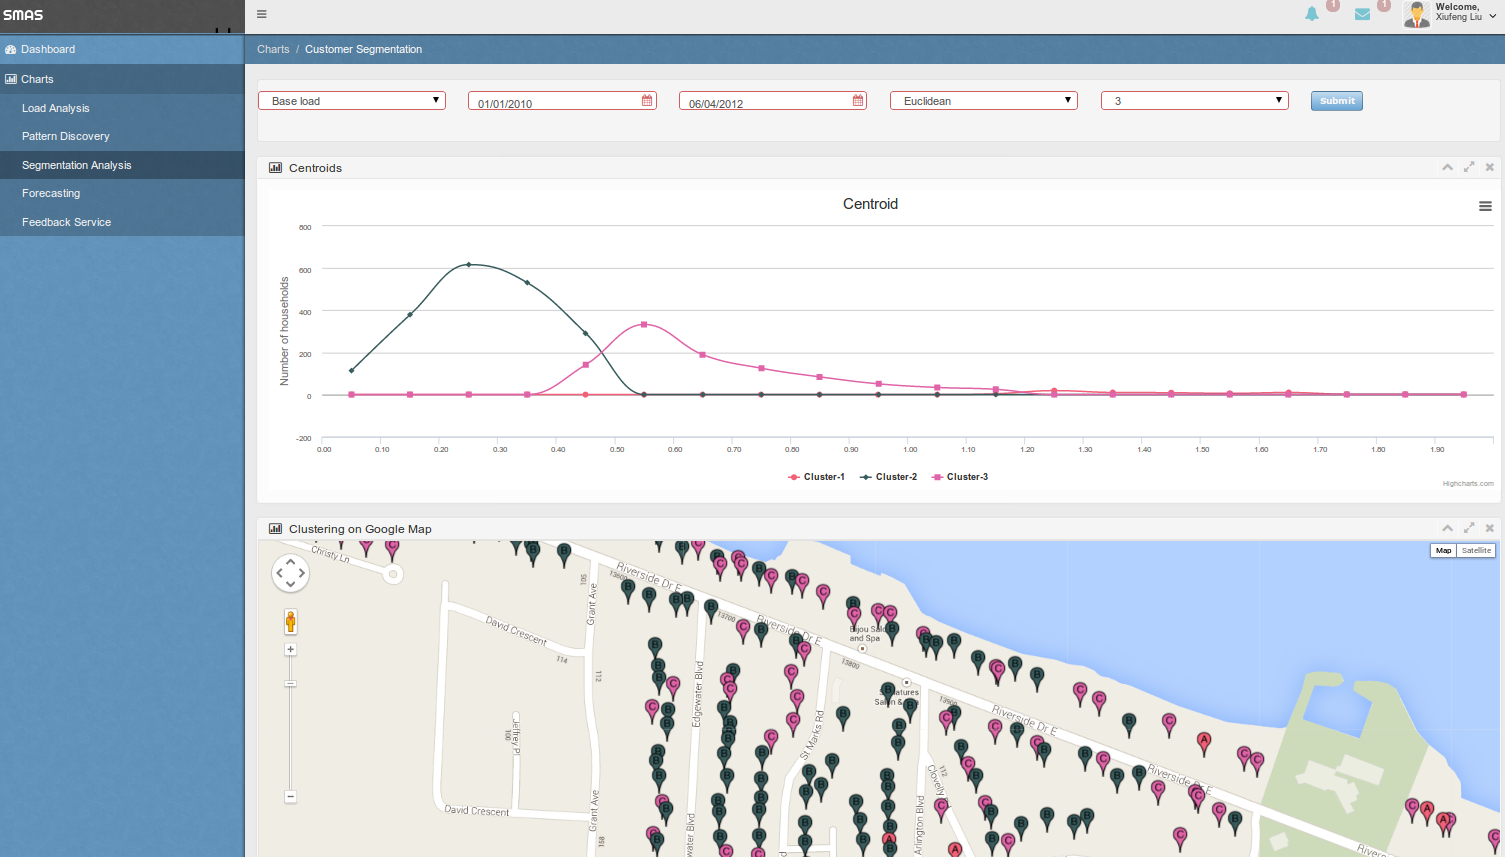
\includegraphics[width=0.82\textwidth]{images/segmentation}
\vspace{-10pt}
\caption{Segmentation}
\label{fig:segmentation}
\vspace{-5pt}
\end{figure*}
\end{document}
